\appendix

\section{Full Per-Seed Results}
\label{app:per-seed}

This appendix reports the per-seed values that underlie the aggregated tables in the main paper. All EuroSAT runs use 50 epochs; BigEarthNet-S2 runs use 15 epochs. Seeds are $\{42, 123, 456\}$ throughout.

\subsection{EuroSAT Per-Seed Overall Accuracy}

\begin{table}[h]
\centering
\small
\caption{EuroSAT per-seed overall accuracy. Each cell is a single training run.}
\label{tab:eurosat-per-seed}
\begin{tabular}{llccc}
\toprule
Method & Modality & seed=42 & seed=123 & seed=456 \\
\midrule
\multirow{5}{*}{Linear Probe}
 & s2\_full   & 0.6589 & 0.6543 & 0.6572 \\
 & rgb        & 0.5570 & 0.5594 & 0.5519 \\
 & rgb\_sar   & 0.5544 & 0.5531 & 0.5498 \\
 & gf2        & 0.6452 & 0.6457 & 0.6559 \\
 & sar\_only  & 0.3870 & 0.3833 & 0.3913 \\
\midrule
\multirow{5}{*}{BitFit}
 & s2\_full   & 0.6996 & 0.7026 & 0.7035 \\
 & rgb        & 0.6076 & 0.6089 & 0.6067 \\
 & rgb\_sar   & 0.6072 & 0.6039 & 0.6052 \\
 & gf2        & 0.7004 & 0.7019 & 0.6998 \\
 & sar\_only  & 0.4470 & 0.4480 & 0.4524 \\
\midrule
\multirow{5}{*}{LoRA (r=8)}
 & s2\_full   & 0.6604 & 0.6548 & 0.6576 \\
 & rgb        & 0.5546 & 0.5596 & 0.5546 \\
 & rgb\_sar   & 0.5557 & 0.5530 & 0.5504 \\
 & gf2        & 0.6444 & 0.6480 & 0.6563 \\
 & sar\_only  & 0.3913 & 0.3831 & 0.3900 \\
\midrule
\multirow{5}{*}{Houlsby}
 & s2\_full   & 0.8189 & 0.8207 & 0.8241 \\
 & rgb        & 0.7294 & 0.7278 & 0.7244 \\
 & rgb\_sar   & 0.7389 & 0.7361 & 0.7387 \\
 & gf2        & 0.8226 & 0.8198 & 0.8178 \\
 & sar\_only  & 0.6111 & 0.6161 & 0.6191 \\
\midrule
\multirow{2}{*}{LoRA Split-QKV}
 & s2\_full   & 0.7093 & 0.7080 & 0.7037 \\
 & rgb        & 0.4969 & 0.4922 & 0.5035 \\
\midrule
\multirow{2}{*}{GeoAdapter v2}
 & s2\_full   & 0.5494 & 0.4607 & 0.4448 \\
 & rgb        & 0.3878 & 0.3956 & 0.3659 \\
\midrule
Full Fine-Tuning & s2\_full & 0.8685 & --- & --- \\
\bottomrule
\end{tabular}
\end{table}

\subsection{BigEarthNet-S2 Per-Seed mAP}

\begin{table}[h]
\centering
\small
\caption{BigEarthNet-S2 per-seed validation mAP (19-class multi-label).}
\label{tab:bigearthnet-per-seed}
\begin{tabular}{llccc}
\toprule
Method & Modality & seed=42 & seed=123 & seed=456 \\
\midrule
\multirow{2}{*}{Linear Probe}
 & s2\_full   & 0.3578 & 0.3606 & 0.3548 \\
 & rgb        & 0.3344 & 0.3343 & 0.3363 \\
\midrule
\multirow{2}{*}{LoRA (r=8)}
 & s2\_full   & 0.3582 & 0.3606 & 0.3545 \\
 & rgb        & 0.3346 & 0.3350 & 0.3363 \\
\midrule
\multirow{2}{*}{Houlsby}
 & s2\_full   & 0.4927 & 0.4815 & 0.4979 \\
 & rgb        & 0.4531 & 0.4583 & 0.4559 \\
\bottomrule
\end{tabular}
\end{table}

\section{Trainable Parameter Budgets}
\label{app:params}

Table~\ref{tab:params} reports the exact trainable parameter count per method, isolated from the frozen Prithvi-100M backbone. The classification head accounts for 7{,}690 parameters on EuroSAT (10 classes) and 14{,}611 on BigEarthNet-S2 (19 classes).

\begin{table}[h]
\centering
\small
\caption{Trainable parameter counts (head included).}
\label{tab:params}
\begin{tabular}{lrr}
\toprule
Method & EuroSAT & BigEarthNet \\
\midrule
Linear Probe       &      7{,}690 &     14{,}611 \\
GeoAdapter v2      &      7{,}873 &        --- \\
BitFit             &    110{,}602 &        --- \\
LoRA (r=8)         &    155{,}146 &    162{,}067 \\
LoRA Split-QKV     &    597{,}514 &        --- \\
Houlsby (d=64)     &  1{,}197{,}322 &  1{,}204{,}243 \\
Full Fine-Tuning   & 86{,}244{,}874 &        --- \\
\bottomrule
\end{tabular}
\end{table}

\section{Training Curves}
\label{app:curves}

Figure~\ref{fig:curve-eurosat} compares the training loss trajectories of full fine-tuning and split-QKV LoRA on EuroSAT s2\_full. Full fine-tuning converges to a substantially lower loss, consistent with its higher final accuracy. Figure~\ref{fig:curve-ben} shows the BigEarthNet-S2 loss curves for the three methods evaluated on that dataset; Houlsby separates from the LoRA/linear-probe cluster early in training.

\begin{figure}[h]
\centering
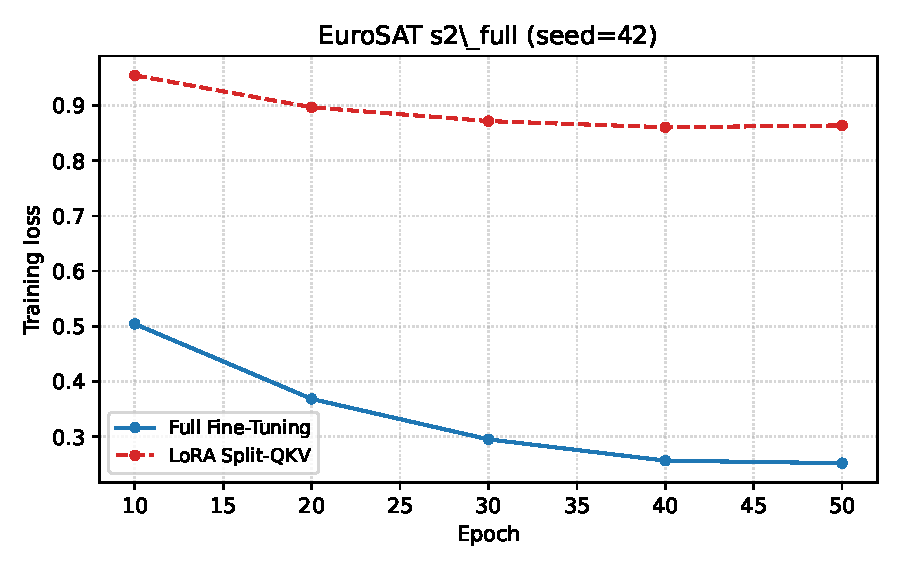
\includegraphics[width=0.85\linewidth]{figures/training_curves_eurosat.pdf}
\caption{Training loss on EuroSAT s2\_full (seed=42). Full fine-tuning reaches a much lower loss floor than split-QKV LoRA.}
\label{fig:curve-eurosat}
\end{figure}

\begin{figure}[h]
\centering
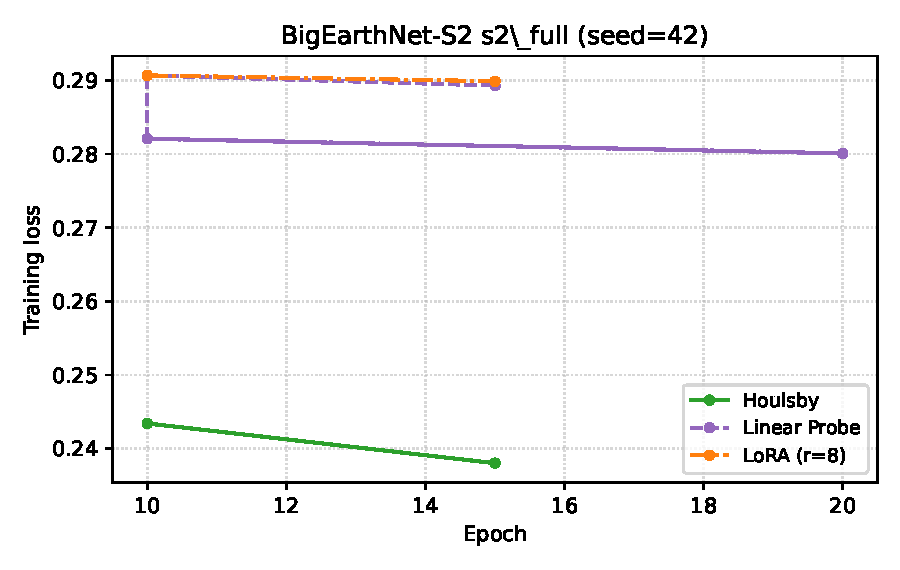
\includegraphics[width=0.85\linewidth]{figures/training_curves_bigearthnet.pdf}
\caption{Training loss on BigEarthNet-S2 s2\_full (seed=42). Houlsby separates from LoRA and linear probing by epoch 10.}
\label{fig:curve-ben}
\end{figure}

\section{Hyperparameters and Compute}
\label{app:hparams}

\paragraph{Optimizer and schedule.}
All runs use AdamW~\cite{loshchilov2019adamw} with cosine annealing~\cite{loshchilov2017sgdr}. Weight decay is $10^{-4}$. The PEFT-parameter learning rate is $10^{-3}$ on EuroSAT and $5\times 10^{-4}$ on BigEarthNet-S2; the classification head receives $5\times 10^{-3}$ throughout. Full fine-tuning uses a single learning rate of $5\times 10^{-5}$.

\paragraph{Batching.}
Standard PEFT runs use batch size 64. Full fine-tuning uses batch size 32 to fit within 40\,GB of A100 memory. BigEarthNet uses batch size 64 for all methods.

\paragraph{Compute.}
All experiments run on a single NVIDIA A100 40\,GB on Google Colab Pro+. Wall-clock time per run averages 19--23 minutes on EuroSAT and 28--34 minutes on BigEarthNet (15 epochs over the 10K subsample). Total compute for the 100 reported runs is approximately 38 GPU-hours.

\paragraph{Data preparation.}
EuroSAT patches are resized from $64\times 64$ to $224\times 224$ and standardized per-band against statistics computed on the training split. BigEarthNet patches are decoded from the GeoTIFF format, resized to $120\times 120$ and standardized identically. Channel zero-padding is applied at the dataloader level to bridge any modality with fewer than 6 channels to Prithvi's 6-channel input expectation.

\section{LoRA Rank Sensitivity}
\label{app:lora-rank}

To test whether the split-QKV LoRA result is merely limited by an underpowered rank choice, we ran an additional ablation on EuroSAT s2\_full with $r\in\{4,8,16,32\}$. The corresponding trainable parameter counts are 302{,}602, 597{,}514, 1{,}187{,}338, and 2{,}366{,}986. The mean overall accuracies (3 seeds each) are 0.7089 $\pm$ 0.0018 ($r=4$), 0.7070 $\pm$ 0.0029 ($r=8$), 0.7069 $\pm$ 0.0013 ($r=16$), and 0.7064 $\pm$ 0.0017 ($r=32$). Figure~\ref{fig:lora-rank} in the main paper visualizes this trend.

The result is qualitatively stable: increasing the LoRA rank does not produce monotonic gains and never approaches the Houlsby adapter score of 0.821. This makes the post-fix LoRA ceiling much harder to dismiss as a hyperparameter artifact. Within the explored budget range, the limitation appears architectural rather than rank-bound.

\section{LoRA Implementation Details and the Fused-QKV Trap}
\label{app:lora-trap}

This section documents the exact code-level cause of the LoRA failure observed in the main paper, since reproducing or refuting our negative result requires reproducing the same insertion pattern.

Prithvi-100M's attention block is implemented as a \texttt{torch.nn.MultiheadAttention} module. In PyTorch's reference implementation, the query, key, and value projections are stored as a single tensor:

\begin{verbatim}
attn.in_proj_weight        # shape [3*D, D]
attn.in_proj_bias          # shape [3*D]
attn.out_proj.weight       # shape [D, D]
attn.out_proj.bias         # shape [D]
\end{verbatim}

A naive LoRA insertion that iterates \texttt{module.named\_modules()} and wraps every \texttt{nn.Linear} child therefore touches only \texttt{out\_proj}: the actual Q, K, V projections are not children of \texttt{MultiheadAttention} and are silently skipped. Training proceeds, loss decreases, and accuracy settles a few hundredths above linear probing --- which is exactly what we observe.

Our split-QKV variant resolves this by replacing each \texttt{MultiheadAttention} with three explicit \texttt{nn.Linear} projections initialized from the corresponding slices of \texttt{in\_proj\_weight}/\texttt{in\_proj\_bias}, then injecting LoRA into each of \texttt{q\_proj}, \texttt{k\_proj}, \texttt{v\_proj}, and \texttt{out\_proj}. The forward pass is rewritten to call each projection separately and re-combine the outputs through the standard scaled dot-product attention. We verified numerical equivalence on a small input batch before training begins.

We emphasize that this is not a bug in any specific PEFT library --- it is a direct consequence of how PyTorch fuses attention projections by default. Any LoRA implementation that targets \texttt{nn.Linear} child modules will silently miss them on Prithvi-100M and other Vision Transformer codebases that build on \texttt{nn.MultiheadAttention}.

\section{LandCover.ai Per-Seed Segmentation Results}
\label{app:seg-per-seed}

\begin{table}[h]
\centering
\small
\caption{LandCover.ai per-seed mIoU. Each cell is a single training run (50 epochs, batch size 8, RGB modality).}
\label{tab:landcoverai-per-seed}
\begin{tabular}{lcccc}
\toprule
Method & Trainable Params & seed=42 & seed=123 & seed=456 \\
\midrule
Linear Probe & 4{,}614       & 0.2508 & 0.2513 & 0.2507 \\
LoRA (r=8)   & 152{,}070     & 0.2511 & 0.2511 & 0.2509 \\
Houlsby      & 1{,}194{,}246 & 0.6392 & 0.6394 & 0.6444 \\
\bottomrule
\end{tabular}
\end{table}

The LoRA and linear-probe seed spreads agree to the fourth decimal place; the Houlsby spread spans $0.0052$, dominated by the seed=456 run. No seed reverses the overall ordering.

\subsection{Linhe LULC Per-Seed Results}
\label{app:linhe-perseed}

Table~\ref{tab:linhe-perseed} reports per-seed mIoU for the methods reported in Section~\ref{sec:linhe}.

\begin{table}[h]
\centering
\small
\caption{Per-seed mIoU on Linhe LULC 6-class segmentation (geographic scene-level split, Esri 2022 labels).}
\label{tab:linhe-perseed}
\begin{tabular}{lcccc}
\toprule
Method & Trainable Params & seed=42 & seed=123 & seed=456 \\
\midrule
Linear Probe & 4{,}614       & 0.1778 & 0.1796 & 0.1752 \\
BitFit       & 107{,}526     & 0.1977 & 0.2003 & 0.1946 \\
LoRA (r=8, split-QKV) & 152{,}070 & 0.1780 & 0.1788 & 0.1748 \\
Houlsby      & 1{,}194{,}246 & 0.2966 & 0.2971 & 0.2860 \\
GeoAdapter   & 4{,}756       & 0.2514 & 0.2751 & 0.2681 \\
\bottomrule
\end{tabular}
\end{table}

The Linhe seed spreads reproduce two qualitative patterns from the public benchmarks. First, LoRA's per-seed values $\{0.1780, 0.1788, 0.1748\}$ are statistically indistinguishable from linear probing's $\{0.1778, 0.1796, 0.1752\}$ to the fourth decimal place --- the same diagnostic signature of LoRA collapse we observed on EuroSAT (Section~\ref{sec:results}) and LandCover.ai (Appendix~\ref{app:per-seed}). Second, seed variance is small relative to the Houlsby--linear-probe gap: the largest per-seed Houlsby reading ($0.297$) exceeds the largest linear-probe reading ($0.180$) by more than 17 mIoU points, so no choice of seed reverses the ordering. GeoAdapter shows the largest seed spread ($0.024$), consistent with its higher variance reported on EuroSAT.

\subsection{LoveDA Cross-Domain Per-Seed Results and Collapse Diagnostics}
\label{app:loveda-perclass}

Table~\ref{tab:loveda-perseed} reports the 30 per-seed mIoU values that underlie Section~\ref{sec:loveda}.

\begin{table}[h]
\centering
\small
\caption{Per-seed mIoU on LoveDA cross-domain 7-class segmentation. Each cell is one independent training run.}
\label{tab:loveda-perseed}
\begin{tabular}{lccccccc}
\toprule
& & \multicolumn{3}{c}{Urban $\rightarrow$ Rural} & \multicolumn{3}{c}{Rural $\rightarrow$ Urban} \\
\cmidrule(lr){3-5}\cmidrule(lr){6-8}
Method & Params & seed=42 & seed=123 & seed=456 & seed=42 & seed=123 & seed=456 \\
\midrule
Linear Probe & 5{,}383       & 0.0857 & 0.0859 & 0.0857 & 0.0949 & 0.0955 & 0.0955 \\
BitFit       & 127{,}495     & 0.0850 & 0.0852 & 0.0849 & 0.0984 & 0.0986 & 0.0982 \\
LoRA (r=8)   & 152{,}839     & 0.0856 & 0.0854 & 0.0855 & 0.0954 & 0.0951 & 0.0953 \\
Houlsby      & 1{,}195{,}015 & 0.1370 & 0.1397 & 0.1387 & 0.2097 & 0.2130 & 0.2132 \\
GeoAdapter   & 5{,}525       & 0.0854 & 0.0858 & 0.0878 & 0.0990 & 0.1013 & 0.1066 \\
\bottomrule
\end{tabular}
\end{table}

The seed dispersion for the four small-PEFT methods is at the fourth decimal place ($\sigma \le 0.0014$), confirming that the cluster near 0.085 / 0.095 is not a seed artifact. Houlsby's seed dispersion is similarly tight ($\sigma = 0.0014$ U$\rightarrow$R, $\sigma = 0.0019$ R$\rightarrow$U), so the per-method ordering reproduces under all $3 \times 3 = 9$ seed pairings.

\paragraph{Collapse-vs-undertraining diagnostic.} To distinguish ``small PEFT collapses to majority-class prediction'' from ``small PEFT learns weak signal that mIoU under-reports,'' we extended the streaming evaluator to record per-class IoU and the predicted-pixel histogram alongside mIoU, and we ran a single-seed sweep on the U$\rightarrow$R direction with the LoRA budget enlarged 5$\times$ in learning rate (lr$_{\mathrm{peft}}$$=$5$\times 10^{-4}$) and 2$\times$ in epochs (60). The diagnostic config and the extended evaluator are released as \texttt{geoadapter/bench/configs/loveda\_lulc\_u2r\_diag.yaml} and \texttt{geoadapter/engine/evaluator.py} respectively. Table~\ref{tab:loveda-diag} reports the per-class IoU vector and the dominant-prediction share recovered by the diagnostic sweep.

\begin{table}[h]
\centering
\small
\caption{LoveDA U$\rightarrow$R diagnostic sweep (single seed, 60 epochs, lr$_{\mathrm{peft}}$$=$5$\times 10^{-4}$). Per-class IoU columns 0--6 follow the LoveDA taxonomy: 0 background, 1 building, 2 road, 3 water, 4 barren, 5 forest, 6 agriculture. ``dom\%'' is the share of validation pixels assigned to the dominant predicted class.}
\label{tab:loveda-diag}
\begin{tabular}{lccccccccr}
\toprule
Method & Params & 0 & 1 & 2 & 3 & 4 & 5 & 6 & dom\% \\
\midrule
LoRA r=8  diag & 152{,}839 & 0.397 & 0.201 & 0.000 & 0.001 & 0.010 & 0.021 & 0.000 & 87.8 \\
LoRA r=16 diag & 300{,}295 & 0.396 & 0.201 & 0.000 & 0.001 & 0.010 & 0.022 & 0.000 & 87.7 \\
\bottomrule
\end{tabular}
\end{table}

The signature is consistent across LoRA ranks: both diagnostic runs recover the building class (IoU $\approx 0.20$) at the cost of background IoU dropping from the all-bg ceiling of $0.60$ to $0.40$, while five of the seven classes (road, water, barren, forest, agriculture) remain at zero IoU. The dominant-prediction share falls from the all-bg ceiling of $\approx$$100\%$ to $\approx$$88\%$, confirming that the model is no longer in pure majority-class collapse, but the class diversity it has learned is exactly two. Doubling LoRA's rank and quadrupling its trainable-parameter budget over the protocol-default schedule yields a +$0.0046$ mIoU gain (best diagnostic mIoU $0.0901$ vs.\ Phase~2 mean $0.0855$), which we read as ruling out undertraining as the explanation for the small-PEFT plateau: the optimization budget is not the bottleneck, the per-method parameter budget is. We retain the term ``capacity threshold'' for the gap between sub-$10^6$ adapters (binary discrimination only) and Houlsby at $\approx$$1.2 \times 10^6$ parameters (non-degenerate IoU on all seven classes).

\section{Reproducibility}
\label{app:repro}

Source code, training logs, raw experiment JSON files, and the figure-generation script are released under the project repository. Each experiment record contains the method name, modality, random seed, trainable parameter count, and metric values. Aggregated tables in the main paper can be reconstructed from these records using \texttt{paper12/scripts/make\_figures.py} and \texttt{summary.csv}.
